\documentclass[twocolumn]{class}


\addbibresource{References.bib}

% add path to images
\graphicspath{ {./images/} }

\title{Heart Disease Prediction from heart beat audio signals using Machine Learning and Network Analysis}
\shorttitle{Heart Disease Prediction}

\github{https://github.com/DavideLigari01/advanced-biomedical-project}

\author{Ligari D. • Alberti A.  }

\affil[1]{Department of Computer Engineering, Data Science, University of Pavia, Italy \newline\centering Course of Advanced Biomedical Machine Learning}

\keywords{---TO BE DEFINED---}
\abstract{  
   Heart disease remains one of the leading causes of mortality worldwide, making early diagnosis crucial. This study aims to predict heart diseases by analyzing heartbeat audio signals using machine learning and network analysis. We utilized a dataset from the PASCAL Classifying Heart Sounds Challenge 2011, which includes normal heart sounds, murmurs, extra heart sounds, extra systoles, and artifacts. Various preprocessing techniques such as noise reduction, resampling, and segmentation were applied to ensure data quality. Features were extracted using methods like Mel-Frequency Cepstral Coefficients (MFCC), Chroma, RMS, ZCR, and spectral features. Multiple machine learning models including LightGBM, XGBoost, CatBoost, Random Forest, and Multilayer Perceptron were trained and evaluated. The best performing model achieved high accuracy in distinguishing between different heart sound categories. This research highlights the potential of machine learning in cardiac diagnostics and provides a foundation for future advancements in the field.
   }
\firstauthor{Alberti Ligari}
\publicationdate{\today}


\begin{document}

\maketitle
\pagestyle{FirstPage}

\tableofcontents
% \nocite{dizdar_dns_2021}

% ------------------- START OF SECTIONS -------------------


% ------------------- Introduction -------------------

\section{Introduction}
Cardiovascular diseases (CVDs) are the leading cause of death globally. Early detection and diagnosis are vital for effective treatment and management of heart conditions. Traditional diagnostic methods, while effective, are often invasive and require significant time and expertise. Recent advancements in machine learning (ML) and signal processing have opened new avenues for non-invasive and rapid diagnosis. This study focuses on the use of ML techniques to analyze heartbeat audio signals and predict the presence of heart diseases.

The dataset used in this study was sourced from the PASCAL Classifying Heart Sounds Challenge 2011. It includes recordings of normal heart sounds, murmurs, extra heart sounds, extra systoles, and artifacts. The primary aim of this research is to develop a robust ML model capable of accurately classifying these heart sounds, thereby aiding in the early diagnosis of various cardiac conditions.

\subsection{Problem Domain}
Despite the advances in medical technology, early and accurate diagnosis of heart diseases remains challenging. Traditional methods such as electrocardiograms (ECG) and echocardiograms, while accurate, are resource-intensive. There is a significant gap in developing accessible, non-invasive diagnostic tools that can provide quick and accurate results.

\subsection{Research Question}
This study addresses the gap by leveraging machine learning techniques to analyze heart sound recordings. The research question is: "How can machine learning models be utilized to classify different types of heart sounds accurately, and which features contribute most significantly to the classification performance?"

\section{Methods}
\subsection{Source of Data}
The dataset for this project was obtained from a Kaggle repository titled \textit{Dangerous Heartbeat Dataset (DHD)} \cite{Dangerous-Heartbeat-Dataset-DHD}, 
which in turn sources its data from the PASCAL Classifying Heart Sounds Challenge 2011 (CHSC2011) \cite{pascal-chsc-2011}. 
This dataset comprises audio recordings of heartbeats, categorized into different types of heart sounds.
Specifically, the dataset consists of 5 types of recordings: Normal Heart Sounds, Murmur Sounds, Extra Heart Sounds, Extrasystole Sounds, and Artifacts.
Data has been gathered from the general public via the iStethoscope Pro iPhone app and from a clinic trial in hospitals using the digital stethoscope DigiScope.

\subsubsection{Data Distribution}
Figure \ref{fig:DataExp_num_durations}, show the presence of highly imbalanced classes in the dataset.
This poses a challenge for the classification task as the model may not have enough samples to learn from,
especially for the 'Extrastole' and 'Extrahls' classes. This problem is tackled trying to augment the data available,
both by segmenting the audio files and by using data augmentation techniques. Furthermore, 
we test the effectiveness of oversampling and undersampling techniques on the model performance.
The data is split intro training and testing sets, with a 80\% - 20\% ratio, respectively. The validation set
is omitted, due to the low number of samples available.

\begin{figure}[H]
    \centering
    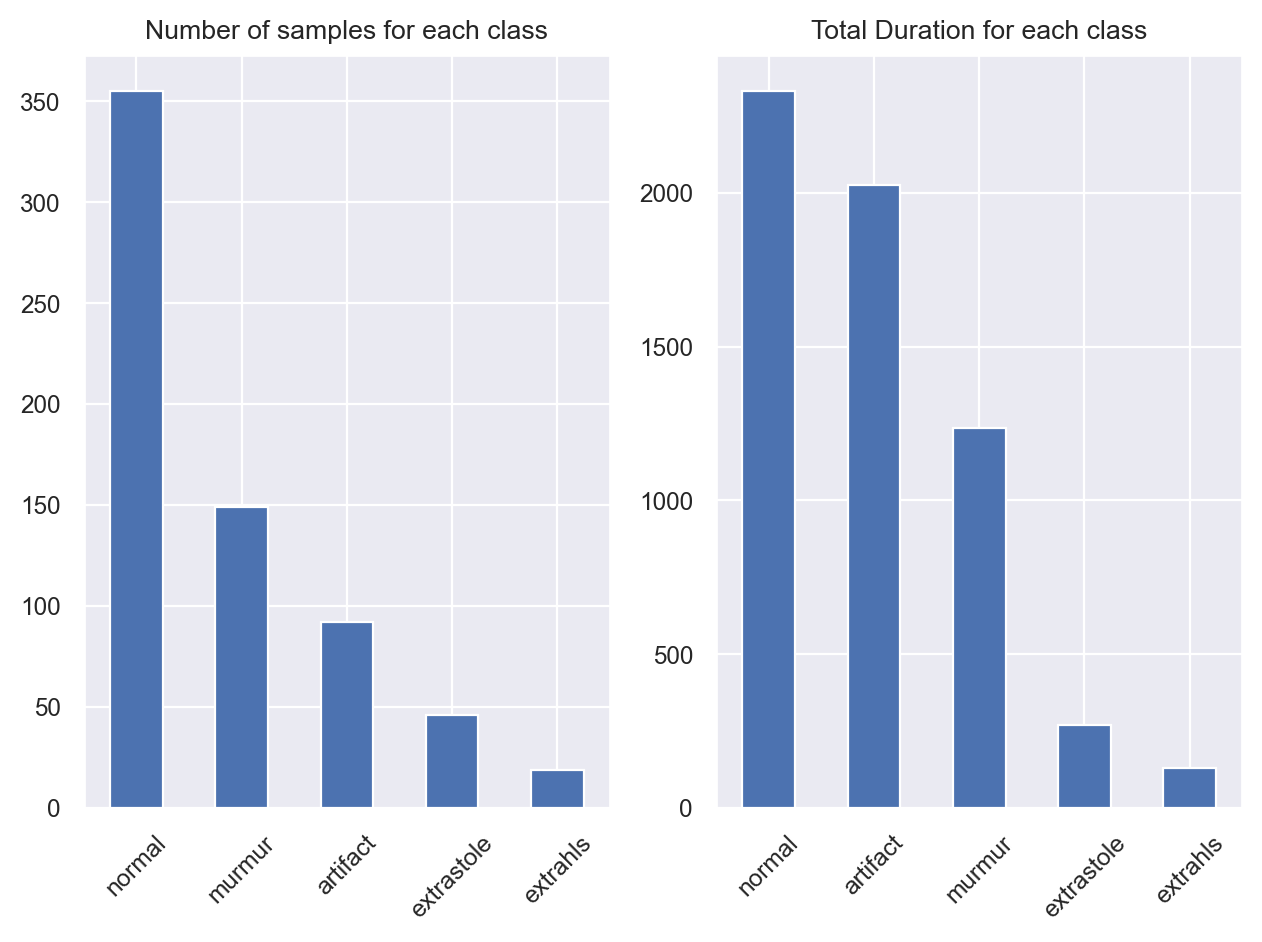
\includegraphics[width=1\columnwidth]{./images/DataExp_num_durations.png}
    \caption{Number of samples per duration.}
    \label{fig:DataExp_num_durations}
\end{figure}



\subsubsection{Data Preprocessing}
Here is a list of the preprocessing operations performed on the dataset:

\vspace{0.3cm}\noindent
\textbf{Noise Reduction:} the audio data was already provided in a clipped format 
to minimize noise and irrelevant information.

\vspace{0.3cm}\noindent
\textbf{Removal of Corrupted Files:} corrupted files were identified and removed 
from the dataset to ensure data quality.

\vspace{0.3cm}\noindent
\textbf{Resampling:} all audio files were resampled to a common frequency of 4000 Hz, 
which was identified as the optimal sampling rate (see Section \ref{sec:sr_extraction_interval}).

\vspace{0.3cm}\noindent
\textbf{Segmentation:} the audio data was segmented into 1-second intervals, 
identified as the optimal extraction interval (see Section \ref{sec:sr_extraction_interval}).

\vspace{0.3cm}\noindent
\textbf{Outlier Detection and Removal:} we investigated the average duration of 
each class and found that the 'artifact' class had a significantly larger average 
duration. This was due to a few lengthy audio 
recordings (see Figure \ref{fig:DataExp_outliers_Artifacts}). These recordings were 
considered as outliers and removed from the dataset, as a large number of samples from 
the same audio might not be as informative.

\begin{figure}[H]
	\centering
	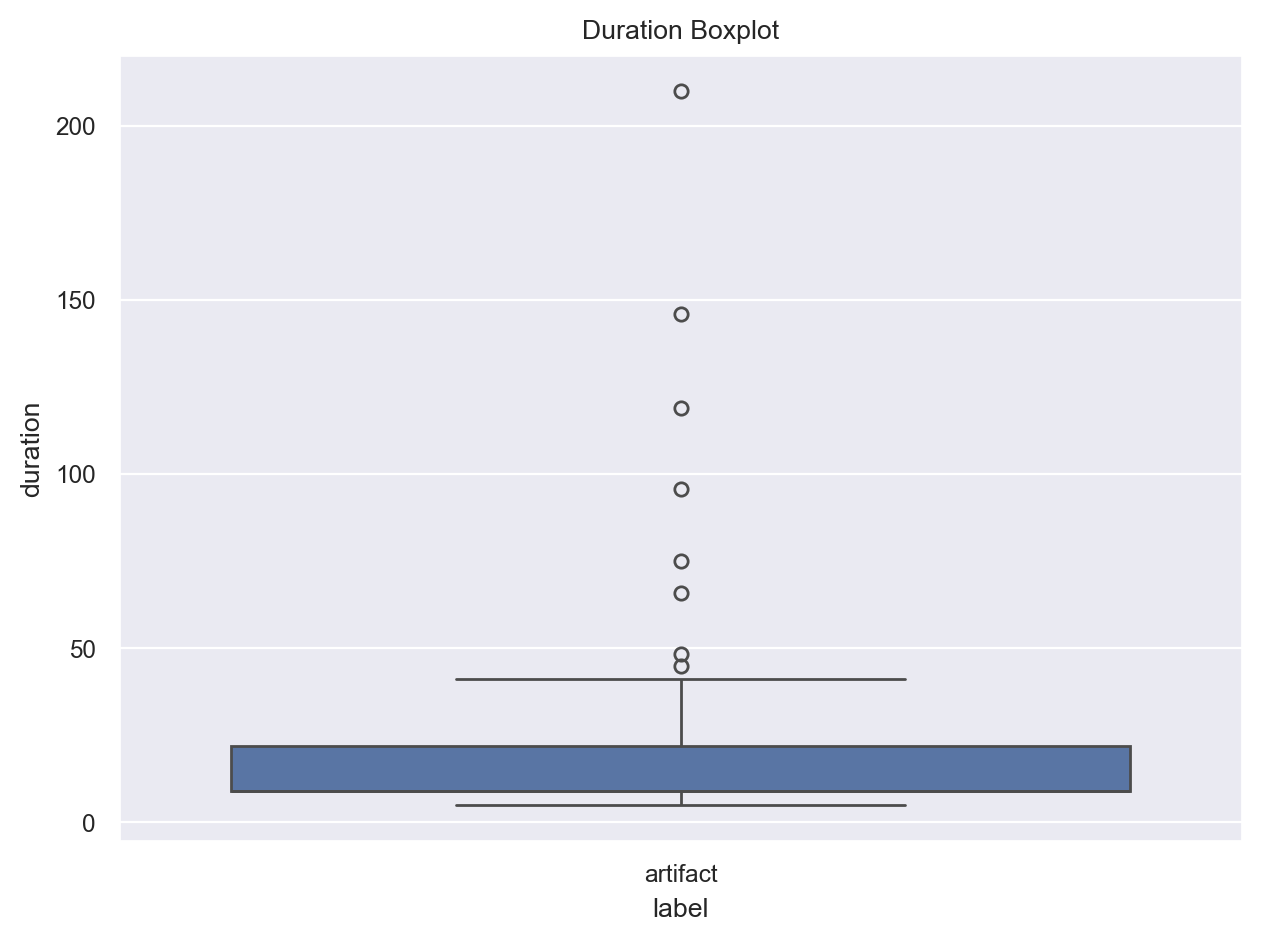
\includegraphics[width=1\columnwidth]{./images/DataExp_outliers_artifact.png}
	\caption{Outliers in the Artifacts class.}
	\label{fig:DataExp_outliers_Artifacts}
 \end{figure}

\subsection{Feature Extraction}
As demonstrated by \cite{Raza_Mehmood_Ullah_Ahmad_Choi_On_2019} and \cite{Chen_Sun_Chen_Xie_Wu_Xu_2021}, MFCCs 
are highly effective features for heartbeat classification. In addition to MFCCs, 
we incorporated other features to capture various characteristics of heart sounds, enhancing the classification accuracy.
The features used are explained in the following section.

\subsubsection{Features Type}

\textbf{MFCC}\newline
Mel-Frequency Cepstral Coefficients (MFCCs) are representations of the short-term power spectrum of sound. 
They are derived by taking the Fourier transform of a signal, mapping the powers of the spectrum onto the mel 
scale, taking the logarithm, and then performing a discrete cosine transform. MFCCs are effective in capturing 
the timbral texture of audio and are widely used in speech and audio processing due to 
their ability to represent the envelope of the time power spectrum.
In heartbeat classification, MFFCs can reflect the different perceived quality of heart sounds,
such as the presence of murmurs or other anomalies.

\vspace{0.5cm}\noindent
\textbf{Chroma STFT}\newline
Chroma features represent the 12 different pitch classes of music (e.g., C, C\#, D, etc.). 
They are particularly useful for capturing harmonic and melodic characteristics in music. 
By mapping audio signals onto the chroma scale, these features can identify pitches regardless 
of the octave, making them useful for analyzing harmonic content in heart sounds.

\vspace{0.5cm}\noindent
\textbf{RMS}\newline
Root Mean Square (RMS) measures the magnitude of varying quantities, in this case, 
the amplitude of an audio signal. It is a straightforward way to compute the energy of 
the signal over a given time frame. RMS is useful in audio analysis for detecting volume 
changes and can help identify different types of heartbeats based on their energy levels.
For example, in a given timeframe the RMS may be altered by the presence of a murmur
with respect to a normal heart sound.

\vspace{0.5cm}\noindent
\textbf{ZCR}\newline
Zero-Crossing Rate (ZCR) is the rate at which a signal changes sign, indicating how often the signal 
crosses the zero amplitude line. It is particularly useful for detecting the noisiness and the temporal 
structure of the signal. In heartbeat classification, ZCR can help differentiate between normal and abnormal 
sounds by highlighting changes in signal periodicity.

\vspace{0.5cm}\noindent
\textbf{CQT}\newline
Constant-Q Transform (CQT) is a time-frequency representation with a logarithmic frequency scale, making it 
suitable for musical applications. Since it captures more detail at lower frequencies, it may be useful for analyzing 
the low-frequency components of heart sounds.

\vspace{0.5cm}\noindent
\textbf{Spectral Centroid}\newline
The spectral centroid indicates the center of mass of the spectrum and is often perceived as the brightness of a 
sound. It is calculated as the weighted mean of the frequencies present in the signal, with their magnitudes as 
weights. In heart sound analysis, a higher spectral centroid can indicate sharper, more pronounced sounds, 
while a lower centroid suggests smoother sounds. 

\vspace{0.5cm}\noindent
\textbf{Spectral Bandwidth}\newline
Spectral bandwidth measures the width of the spectrum around the centroid, providing an indication of the range 
of frequencies present. It is calculated as the square root of the variance of the spectrum. This feature helps 
in understanding the spread of the frequency components in the heart sounds, which can be indicative of different 
heart conditions.

\vspace{0.5cm}\noindent
\textbf{Spectral Roll-off}
Spectral roll-off is the frequency below which a certain percentage of the total spectral energy lies. It is 
typically set at 85\% and helps distinguish between harmonic and non-harmonic content. In heartbeat classification, 
spectral roll-off can be used to differentiate between sounds with a concentrated energy distribution and those with more dispersed energy.

\subsubsection{Methodology}
The features were extracted from the audio signals using the \textit{Librosa} library in Python. It is worth to underline four main aspects in the extraction
methodology having a direct impact on the results:
\begin{itemize}[leftmargin=*]
    \item \textbf{Normalization}: the audio are loaded using the \textit{torchaudio.load()} function, which normalized the audio signals in the range [-1, 1]. This is important to ensure that the features are on the same scale and to prevent the model from being biased towards features with larger values.
    \item \textbf{Audio Clipping}: to extract features, we divided the audio recordings into chunks of a given length (in seconds). This segmentation allowed us to analyze the impact of different extraction intervals on model performance, additionally it allow for augmenting the data available. 
    \item \textbf{Sampling Rate}: while literature on spoken language often suggests that 16000 Hz is sufficient, it was necessary to assess the best sampling rate for heartbeat sounds specifically. We evaluated two sampling rates to determine the optimal rate for heartbeat sounds. 
    \item \textbf{Hop and Window Size}: the hop size determines the number of samples between successive windows, while the window size determines the number of samples considered. Each feature was extracted using the same window length and hop length facilitating a fair assessment of each feature's contribution to the classification task. 
\end{itemize}
The library used for the extraction is \textit{Librosa}, which is a Python package for music and audio analysis. 

\subsubsection{Sampling Rate and Interval Selection} \label{sec:sr_extraction_interval}
To determine the optimal sampling rate and extraction interval for heartbeat classification, a series of experiments was conducted.
We trained various models (Random Forest, Support Vector Machine, Logistic Regression) with different features (Chroma, MFCC\_30, MFCC\_120, CQT\_30, CQT\_70),
sampling rates (mixed, 4000 Hz), and extraction intervals (0.5s, 1s, 2s, 3s). Features were used as extracted without any additional processing. 
The models were trained on 80\% of the data and tested on the remaining 20\%.

\subsubsection{Findings on Sampling Rate}
Our experiments revealed no clear advantage of using a mix of frequencies over a fixed sample rate, independently of the metric used.
Specifically, a fixed sampling rate of 4000 Hz was found to reduce the risk of bias introduction, improve efficiency, 
and enable the use of a wider variety of features. This sampling rate provided a consistent and reliable basis 
for feature extraction, as demonstrated in Figure \ref{fig:sample_rate_impact}.

\begin{figure}[H]
    \centering
    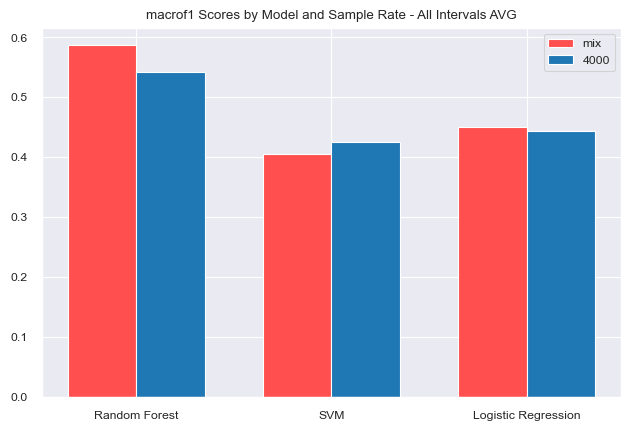
\includegraphics[width=1\columnwidth]{./images/sample_rate_impact.png}
    \caption{Comparison of the macro F1 score for different sampling rates.}
    \label{fig:sample_rate_impact}
\end{figure}

\subsubsection{Findings on Extraction Interval}
The choice of extraction interval had a significant impact on the number of samples and the class distribution, as shown in Figure \ref{fig:interval_class_distribution}.
To address the high class imbalance, we used the macro F1 score and Matthews Correlation Coefficient (MCC) as evaluation metrics. 
Our results indicated that a 2-second interval yielded the best performance. However, this choice also reduced the number of samples, 
potentially causing issues during training and testing, especially with more complex models. 

\begin{figure*}[htbp]
    \centering
    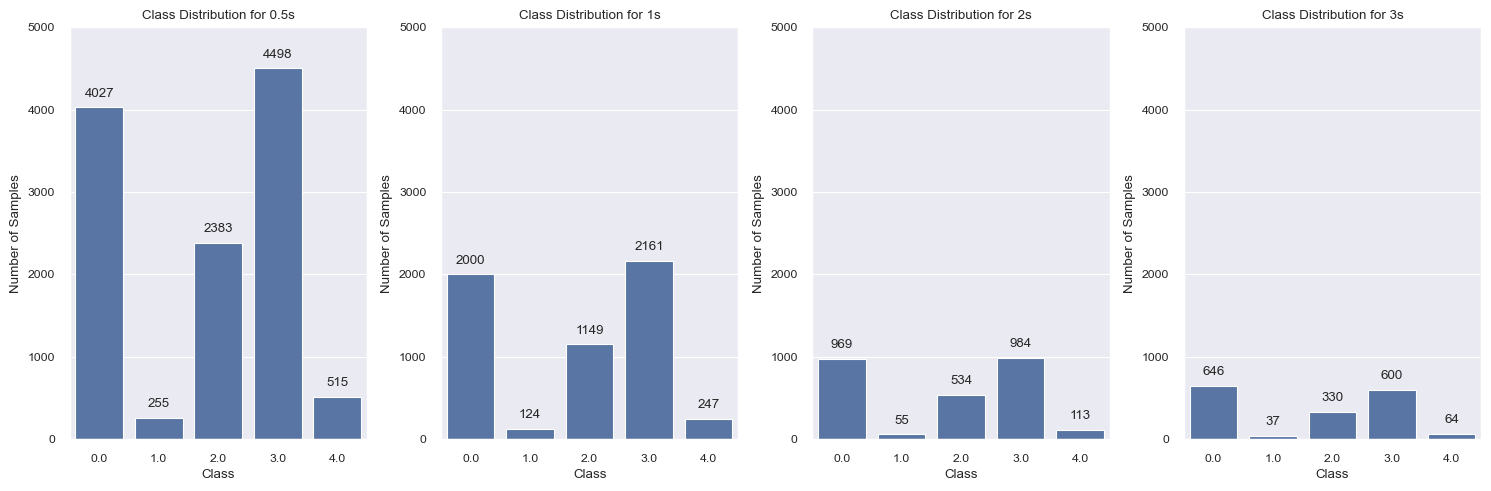
\includegraphics[width=1\textwidth]{./images/interval_class_distribution.png}
    \caption{Class distribution for different extraction intervals.}
    \label{fig:interval_class_distribution}
\end{figure*}

As a compromise, we recommend using a 1-second interval. This interval offers a good balance between 
the number of samples and the class distribution, ensuring robust model performance while maintaining a 
sufficient dataset size. Figures \ref{fig:interval_impact_macrof1} and \ref{fig:interval_impact_mcc} illustrate the impact of 
different extraction intervals on the macro F1 score and MCC, respectively.

\begin{figure}[H]
    \centering
    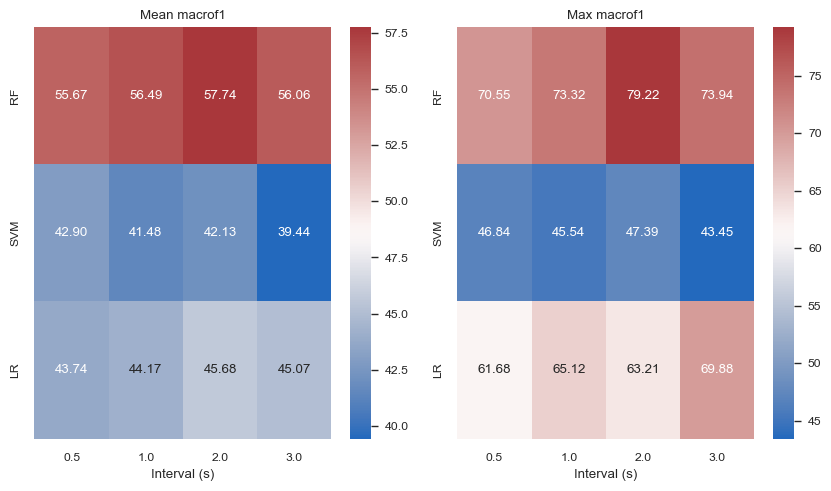
\includegraphics[width=1\columnwidth]{./images/interval_impact_macrof1.png}
    \caption{Comparison of the macro F1 score for different extraction intervals.}
    \label{fig:interval_impact_macrof1}
\end{figure}

\begin{figure}[H]
    \centering
    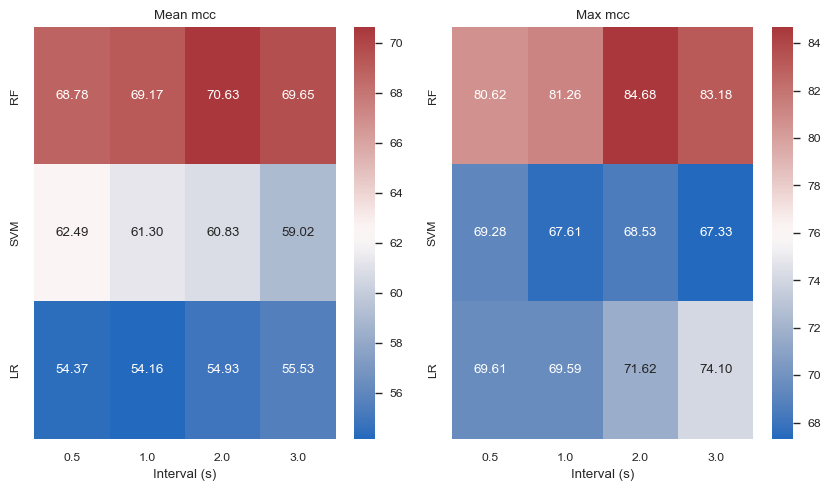
\includegraphics[width=1\columnwidth]{./images/interval_impact_mcc.png}
    \caption{Comparison of the MCC for different extraction intervals.}
    \label{fig:interval_impact_mcc}
\end{figure}


\section{Results}
\subsection{Listing and Evaluation of Results}
The models trained included LightGBM, XGBoost, CatBoost, Random Forest, and Multilayer Perceptron. Each model's performance was evaluated based on accuracy, precision, recall, and F1-score. The best performing model was identified and further analyzed.

\section{Discussion}
\subsection{Positioning in Existing Research}
This study builds on previous work in the field of heart sound classification using machine learning. The results demonstrate the effectiveness of the selected features and models in accurately classifying heart sounds.

\subsection{Limitations}
The primary limitations of this study include the imbalanced dataset and the potential for overfitting due to the relatively small sample size. Future work should focus on acquiring more data and exploring additional feature extraction methods.

\section{Conclusion}
\subsection{Overall Impression}
This research demonstrates the potential of machine learning in the non-invasive diagnosis of heart diseases using audio recordings of heartbeats. The findings suggest that with appropriate preprocessing and feature extraction, ML models can achieve high accuracy in classifying different types of heart sounds.

\subsection{Future Work}
Future research should aim to expand the dataset, explore more advanced feature extraction techniques, and evaluate the models in real-world clinical settings.


\clearpage
\section{Appendix}

% Figure on the best prevention model


% color the image in black
\begin{figure}[H]
    \centering
    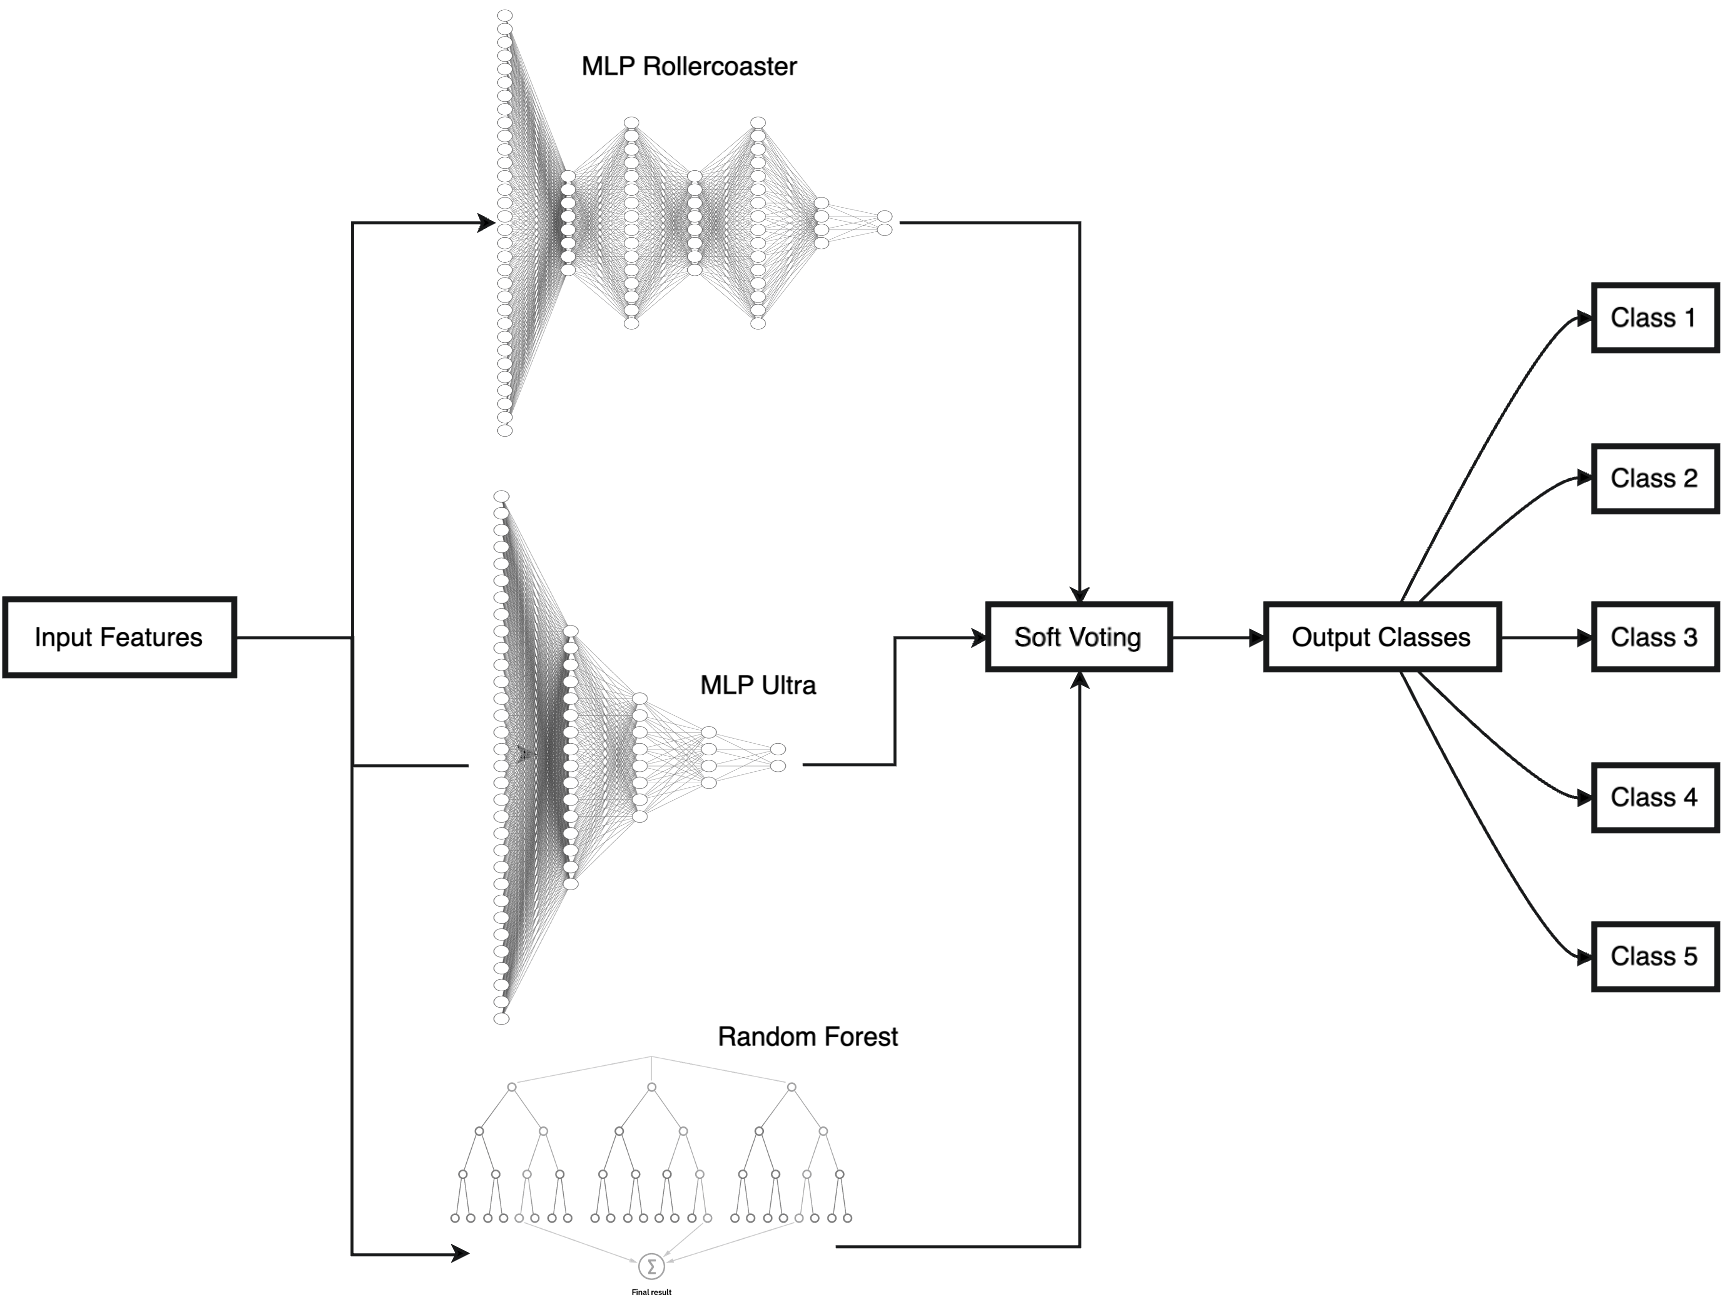
\includegraphics[width=1\columnwidth]{./images/MLP_Ensemble5.png}
    \caption{MLP Ensemble5 Architecture}
    \label{fig:MLP_Ensemble5}
\end{figure}

\clearpage
\printbibliography

\end{document}